\documentclass{article}
\usepackage[final]{nips_2017}
\usepackage[polish]{babel}
\usepackage[utf8]{inputenc} % allow utf-8 input
\usepackage[T1]{fontenc}    % use 8-bit T1 fonts
\usepackage{hyperref}       % hyperlinks
\usepackage{url}            % simple URL typesetting
\usepackage{booktabs}       % professional-quality tables
\usepackage{amsfonts}       % blackboard math symbols
\usepackage{nicefrac}       % compact symbols for 1/2, etc.
\usepackage{microtype}      % microtypography
\usepackage{graphicx}
\graphicspath{ {./images/} }

\title{ Proste sieci neuronowe }

\author{
  Rafał Behrendt \\
  \texttt{246643@student.pwr.edu.pl} \\
  Prowadzący: dr Urszula Markowska \\
  \today
}

\begin{document}

\maketitle

\begin{abstract}
  Celem ćwiczenia jest poznanie podstawowych funkcji wykonywanych przez pojedynczy neuron,
  obserwacja zachowania neuronu przy różnych funkcjach przejścia oraz określenie wielkości, 
  które mają wpływ na szybkość uczenia neuronu. Zrealizowano model perceptronu oraz Adaline.
  Każdy eksperyment testujący wpływ hiperparametrów został przeprowadzony 10-krotnie,
  a wyniki uśredniono. Eksperymenty przeprowadzono na zbiorze testowym zawierającym 30 elementów.
\end{abstract}

\newpage
\section{Eksperymenty}

\subsection{Ręcznie ustawiany bias}

Zbadano ilość wymaganych epok do zakończenia procesu uczenia.
Bias zmieniano krokowo o wartość $0.2$ od $-1$ do $1$. Każdy eksperyment przeprowadzono na przygotwanych
wcześniej wagach wylosowanych z zakresu od $-1$ do $1$. Współczynnik uczenia ustawiono na $\alpha = 0.1$,
a dopuszczalny błąd w Adaline na $0.3$.

\begin{table}[h]
  \centering
    
  \bgroup
  \def\arraystretch{1.3}
  \begin{tabular}{|l|l|l|l|}
  \hline
  Bias & P. bipolar & P. unipolar & Adaline  \\ \hline
  -1 & 11 & 19 & 34 \\ \hline
  -0,8 & 11 & 21 & 35 \\ \hline
  -0,6 & 12 & 20 & 38 \\ \hline
  -0,4 & 12 & 21 & 40 \\ \hline
  -0,2 & 12 & 20 & 44 \\ \hline
  0 & 11 & 18 & 49 \\ \hline
  0,2 & 11 & 18 & 54 \\ \hline
  0,4 & 11 & 18 & 59 \\ \hline
  0,6 & 10 & 19 & 65 \\ \hline
  0,8 & 12 & 21 & 72 \\ \hline
  1 & 13 & 23 & 79 \\ \hline
  Średnia & 11,45455 & 19,81818 & 51,72727 \\ \hline
  \end{tabular}
  \egroup
  \vspace{10px}
  \caption{Ręczny bias}
\end{table}

\begin{figure}[h]
  \centering
  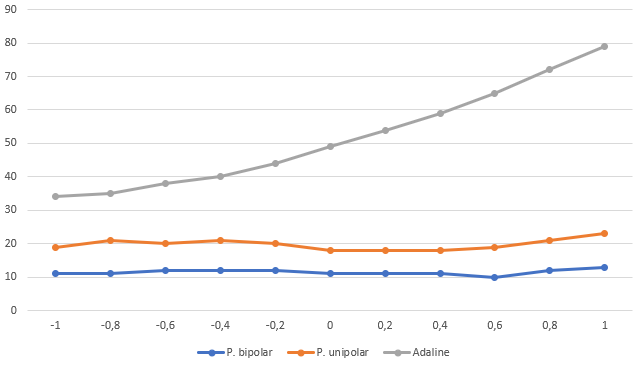
\includegraphics[width=\linewidth]{manualbias.png}
  \caption{Wpływ ręcznie ustawianego biasu na ilość epok}
\end{figure}

\newpage
\subsection{ Testy wpływu zakresu użytych wag }

Zbadano ilość wymaganych epok do zakończenia procesu uczenia. Przeprowadzono 10 eksperymentów, a wyniki uśredniono.
Do przeprowadzenia eksperymentu wykorzystano losowo wygnerowane wagi z krokowo zmieniającego się zakresu.
Współczynnik uczenia ustawiono na $\alpha = 0.1$, a dopuszczalny błąd w Adaline na $0.3$.

\begin{table}[h]
  \centering
    
  \bgroup
  \def\arraystretch{1.3}
  \begin{tabular}{|l|l|l|l|}
  \hline
  Zakres & P. bipolar & P. unipolar & Adaline  \\ \hline
  0,1 & 3,3 & 4,9 & 34,6 \\ \hline
  0,2 & 4,2 & 5,4 & 34,8 \\ \hline
  0,3 & 5,7 & 6,9 & 36,7 \\ \hline
  0,4 & 5,1 & 8,4 & 34,7 \\ \hline
  0,5 & 5,2 & 8,6 & 36,9 \\ \hline
  0,6 & 7,4 & 8,9 & 37,3 \\ \hline
  0,7 & 9,5 & 10,6 & 31,3 \\ \hline
  0,8 & 8,4 & 12,5 & 50,1 \\ \hline
  0,9 & 7,8 & 17,4 & 36,6 \\ \hline
  1 & 7 & 14,3 & 50,3 \\ \hline
  Średnia & 6,36 & 9,79 & 38,33 \\ \hline
  \end{tabular}
  \egroup
  \vspace{10px}
  \caption{Zakres generowanych wag}
\end{table}

\begin{figure}[h]
  \centering
  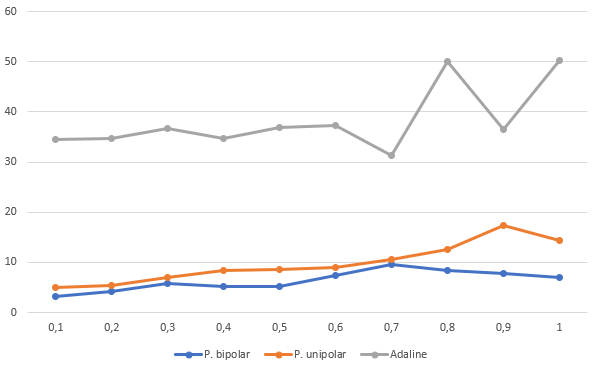
\includegraphics[width=\linewidth]{weights.png}
  \caption{Wpływ zakresu wag na ilość epok}
\end{figure}

\newpage
\subsection{ Testy wpływu współczynnika uczenia }

Zbadano ilość wymaganych epok do zakończenia procesu uczenia. Przeprowadzono 10 eksperymentów, a wyniki uśredniono.
Do przeprowadzenia eksperymentu wykorzystano losowo wygnerowane wagi z krokowo zmieniającego się zakresu.
Współczynnik zmieniano krokowo o wartość $0.05$.
Dopuszczalny błąd w Adaline ustawiono na $0.3$.

\begin{table}[h]
  \centering
    
  \bgroup
  \def\arraystretch{1.3}
  \begin{tabular}{|l|l|l|l|}
  \hline
  Współczynnik uczenia & P. bipolar & P. unipolar & Adaline  \\ \hline
  0,005 & 12 & 34 & 128 \\ \hline
  0,02 & 5 & 12 & 38 \\ \hline
  0,035 & 5 & 8 & 26 \\ \hline
  0,05 & 6 & 6 & 22 \\ \hline
  0,065 & 5 & 6 & 21 \\ \hline
  0,08 & 4 & 6 & 21 \\ \hline
  0,095 & 4 & 5 & 24 \\ \hline
  0,11 & 3 & 4 & 31 \\ \hline
  0,125 & 3 & 5 & 47 \\ \hline
  0,14 & 3 & 5 & 248 \\ \hline
  Średnia & 5 & 9,1 & 60,6 \\ \hline
  \end{tabular}
  \egroup
  \vspace{10px}
  \caption{Zakres generowanych wag}
\end{table}

\begin{figure}[h]
  \centering
  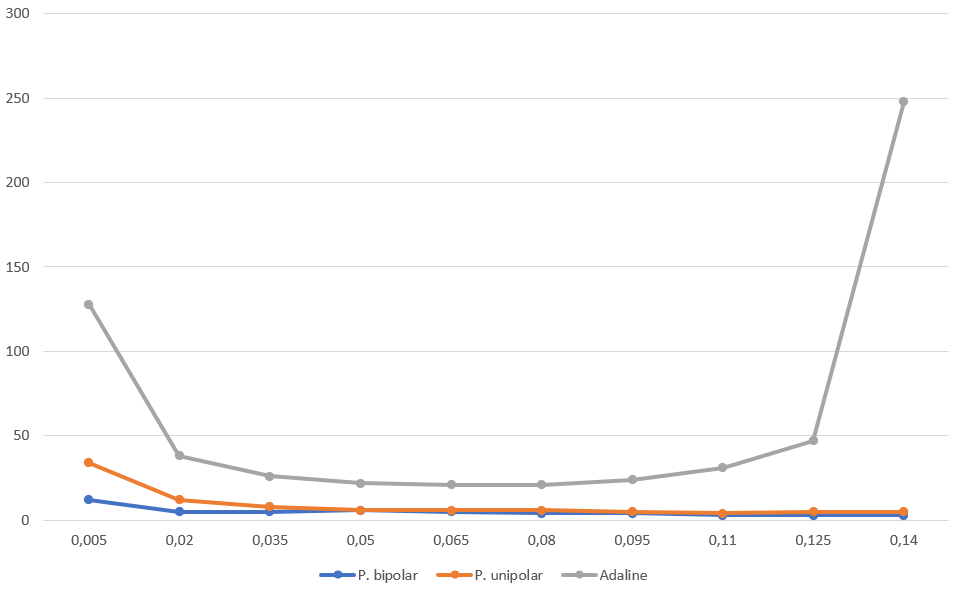
\includegraphics[width=\linewidth]{learnRate.png}
  \caption{Wpłwy współczynnika uczenia na ilość epok}
\end{figure}

\newpage
\subsection{ Ustawienie dopuszczalnego błędu }

Ustawienie odpowiedniego dopuszczalnego błędu wiązało się ze sprawdzeniem jak zmienia się wykres
błędu średniokwadratowego na przestrzeni epok.

\begin{figure}[h]
  \centering
  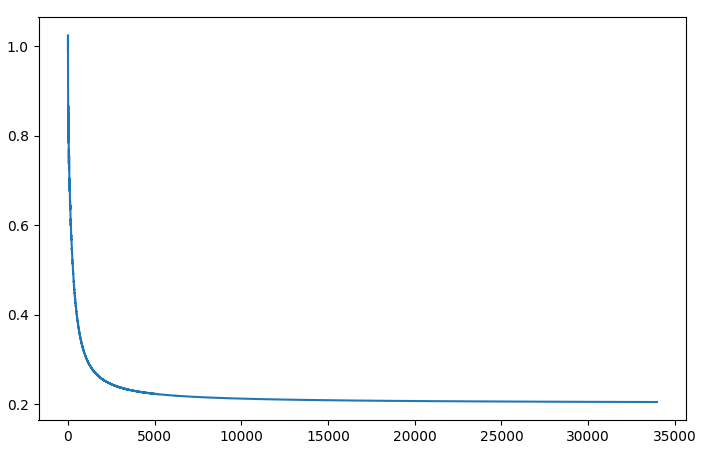
\includegraphics[width=\linewidth]{1000epochs.png}
  \caption{Zmiana błędu średniokwadratowego na przestrzeni epok}
\end{figure}

Z wykresu można odczytać że błąd początkowo mocno spada, po czym następuje zwolnienie. Ustawiono
optymalną wartość $0.3$ na dopusczalny błąd, po którym algorytm kończy działanie. Poniższy wykres przedstawia
zmianę błędu średniokwadratowego do osiągnięcia pożądanego progu. 

\begin{figure}[h]
  \centering
  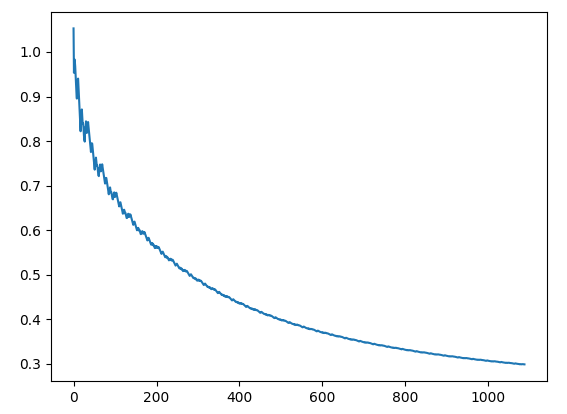
\includegraphics[width=.8\textwidth]{03lr.png}
  \caption{Zmiana błędu średniokwadratowego z dopuszczalnym błędem}
\end{figure}

\section{Wnioski}

W przypadku perceptronu ręczne ustawienie biasu nie ma dużęgo wpływu. Ma on jednak wpływ na działanie
Adaline - im wyższy tym ten dłużej się uczy.

W przypadku dobierania zakresu wag, można zauważyć, że im wyższy przedział, tym algorytmy dłużej się uczą.

Wyniki eksperymentu związanego z dopasowaniem współczynnika uczenia wskazuje, że istnieje pewna wartość
optymalna - dla zbyt niskich, lub zbyt wysokich wartości algorytm uczy się wolniej. Szczególnie dobrze
widać to w przypadku algorytmu Adaline. Należy wiedzieć, że zbyt wysoka wartość może doprowadzić do tego,
że algorytm nigdy się nie nauczy, gdyż może łatwo przeoczyć odpowiednie wartości. Za niska wartość z kolei
daje większą pewność znalezenia dokładnego rozwiązania, jednak może wymagać dużo czasu.

Ustawienie dopuszczalnego błędu w algorytmie Adaline wiąże się z obserwacją zmian. Im błąd wyższy, tym algorytm
szybciej zakończy proces uczenia, może jednak skutkować niedostatecznym nauczeniem. Niski błąd zapewnia większą
dokładność neuronu, jednak może trwać bardzo długo.

\end{document}